% Author: Izaak Neutelings (March 2019)
% Inspiration: https://tex.stackexchange.com/questions/203597/automatically-generate-graphics-which-shows-light-diffusion-on-a-rough-surface
\documentclass[border=3pt,tikz]{standalone}
\tikzset{>=latex} % for LaTeX arrow head
\usetikzlibrary{decorations.pathmorphing,decorations.markings,calc}

\begin{document}

% BLACK BODY
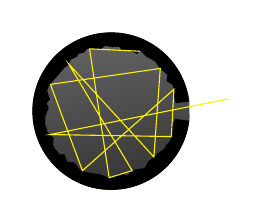
\begin{tikzpicture}
  
  \shade[top color=black!60,bottom color=black!80,shading angle=10]
    (7:1) arc (7:355:1);
  
  \fill[thick,black,postaction=decorate,
    decoration={markings,mark=between positions 0.55 and 1 step 0.03 with {
                  \node[transform shape,inner sep=1pt]
                  (hit\pgfkeysvalueof{/pgf/decoration/mark info/sequence number}) {};
    }}]
    (7:1) arc (7:353:1) --++ (-7:-0.18)
    decorate[decoration={random steps,segment length=2,amplitude=1pt}]
        {arc (-7:-353:0.82)} -- cycle;
  
  \draw[yellow]
    (6:1.5) -- (hit7.center) -- (hit1.center) -- (hit15.center) -- (hit5.center) -- (hit9.center) -- (hit14.center) -- (hit2.center) -- (hit10.center) -- (hit3.center) -- (hit4.center) -- (hit11.center) -- (hit13.center);

\end{tikzpicture}

\end{document}
